%Diese Datei erzeugt die gesamte Hausarbeit.
%Dokumentklasse, die speziell an die Bedürfnisse des Institut mür Musikwissenschaft und Musikinforamtik der Hochschule für Musik Karlsruhe angepasst wurde.
\documentclass[]{../Styles/HfM-KA-IMWI} 

% Sprachpaket
\usepackage[american,british,ngerman]{babel}
% Sprachpakete 1. Deutsch 2. Englisch 3. USenglisch
% Mögl. Optionen für Englisch: [british,UKenglish,USenglish,english,american]

% Anführungszeichen %%Englisch: [babel, british]
\usepackage[babel,german=guillemets]{csquotes}

%Definition der Seitenränder und Sperrvermerke (Ausgelagert in Optionen zur Klasse)
\Seitenraender
\Sperrvermerke

\begin{document}
%Include erzeugt eine neue Seite mit dem Eingebundenen Inhalt
%Deckblatt für Hausarbeiten.

\begin{titlepage}
	\centering
	
	%Logo
	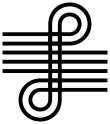
\includegraphics[width=0.15\textwidth]{../Grafiken/Logo_HfM_KA}\par
	
	\vspace{0.6cm}
	
	%Kopfzeile
	{\scshape\LARGE Hochschule für Musik Karlsruhe \par
		\vspace{0.2cm}
		\large Institut für Musikwissenschaft und Musikinformatik\par}
	\vspace{1cm}
	
	%Modul-Angabe
	{\Large \modulname –\modulkuerzel\par}
	
	\vspace{4.5cm}
	
	%Titel
	{\Huge\textbf{\titel}}\par
		{\huge\textsl{\untertitelI\\}}\par
		{\huge\textsl{\untertitelII\\}}
	\vspace{4.5cm}

	%Verfasserangaben
	{
		\textsc{\verfasser} \par
		\vspace{0.4cm}
		\adresse \par
		\email \par}
	\vspace{0.3cm}
	
	%Datum
	{\large \abgabedatum}
\end{titlepage}

%To-Do-Liste (Wird bei Option "druckfreigabe" nicht angezeigt)
\ToDoList

\tableofcontents{\protect \thispagestyle{empty}}

\newpage{}
\setcounter{tocdepth}{2}
\pagenumbering{arabic}
\setcounter{page}{1}
\pagestyle{scrheadings}

%Textinhalt des Dokumentes. Beliebig erweiterbar durch weitere Dateien.
% Benutzt mann \include{file} statt \input{file} wird für jeden include eine neue Seite Begonnen, egal wie viel Platz auf der Seite davor ist. Bei \input{file} wird die Seite normal weitergeführt. \include{file} eignet sich besser für Buch-Kapitel, \include{file} mehr für Artikel und Aufsätze.
\begin{spacing}{1,5}

\IfFileExists{HfM-KA-IMWI-Doku-Vorwort}{\label{Vorwort}%Vorwort

\mysection{0}{Vorwort}

Die Infrastruktur wurde während der Erstellung einer wissenschaftlichen Hausarbeit am Institut für Musikwissenschaft und Musikinformatik an der Hochschule für Musik Karlsruhe entwickelt.
Die vorliegende Struktur ist der Versuch sämtliche eingearbeitete Tools, Umgebungen und Voreinstellung so zu verallgemeinern, dass ein Jeder diese Infrastruktur zum eigenen Bedarf benutzen kann.
Durch die Auslagerung in einzelne Pakete soll gewährleistet sein, dass weitere zusätzliche Erweiterungen für bisher nicht bedachte Fälle, einfach eingebunden werden können.
Auch können dadurch weitere Vorlagen erstellt und nur benötigte Pakete verwendet werden.
Im Folgenden werden nun die Struktur, deren Idee und die einzelnen Pakete genauer erklärt, damit die Funktionsweise verständlich und nachvollziehbar wird.
Diese Dokumentation \underline{kann (leider) nicht} vollständig sein, da jedes einzelne verwendete Paket -- angefangen bei der zugrundeliegenden Dokumentenklasse -- einen derartigen Umfang an Funktionen, Details und Einstellungen besitzt, dass ich mir sicher bin gar nicht alle zu kennen.
Dennoch versuche ich meine Ideen in Worte zu Fassen, um die Gedankengänge, welche ich bei der Erstellung hatte, sichtbar zu machen.

Da ich hauptberuflich Musikwissenschaftler bin und nicht über die Kenntnisse eines Informatikers verfüge und nicht das Feingespür für \enquote{schönes Coden} besitze, bitte ich an dieser Stelle um Entschuldigung bei all denjenigen, die den Code ästhetischer organisiert hätten.
Jedoch ist meine intuitive Gestaltung -- davon bin ich überzeugt -- dahingehend gewinnbringend, dass ich unglaublich viel bei der Programmierung lernen konnte und dass das Ergebnis genau auf die Bedürfnisse eines Studierenden der Hochschule für Musik Karlsruhe angepasst ist.

Für fehlende Funktionen, nicht bedachte Fälle oder mangelnde Dokumentation stehe ich jederzeit gerne beratend zur Verfügung und werde gerne Anregungen und Kritik bei der Weiterentwicklung bedenken.

\begin{flushright}
	Karlsruhe, den \today\\
	\textsc{Dennis Ried}
\end{flushright}}{}
\newpage
\IfFileExists{HfM-KA-IMWI-Doku-Kapitel_01}{\label{Kapitel-01}%Kapitel 1

\section{Aufbau der \LaTeX-Infrastruktur}
\label{sec:AufbauInfrastruktur}

\subsection{Die Ordnerstruktur}
\label{subsec:Ordnerstruktur}
\begin{itemize}
\item Bibliographie: Dieser Ordner enthält die Bibliographie, die der Arbeit zugrunde liegt. In der Regel ist dies eine einzige Datei, aber auch mehrere Dateien sind denkbar. Möchte man ein unterteiltes Literaturverzeichnis einsetzen, kann dies auch über eine \doc{.bib}-Datei geschehen; mehrere Bibliographien sind dafür nicht nötig (s. Bib-Lit.)
\item Dokumentation: Enthält die TeX-Dateien zur Erzeugung dieser Dokumentation. Allerdings nur auf dem Branch \enquote{Dokumentation}.
\item Grafiken: Hier ist der Ort, an dem das Logo für die Titelseite hinterlegt ist. Sinnvoll ist es hier alle die Arbeit betreffenden Bilder zu hinterlegen. Diese können dann ganz einfach über relative Links Eingebunden werden. Selbstverständlich können die Bilder (außer dem Logo) an jedem beliebigen Ort liegen, jedoch erhält man mehr Übersichtlichkeit und Ordnung, wenn man alle an einem Ort sammelt.
\item Interna: Dieser Ordner enthält den Link zum Repository und ist nur vorläufig. Sobald diese Dokumentation fertiggestellt ist wird diese alles notwendige enthalten und dieser Ordner verschwinden.
\item Literatur: Eine der wichtigsten Anlaufstellen zur Erweiterung von \LaTeX-Umgebungen ist das Internet. Wichtige, umfangreiche oder schwer zu findende Dokumentationen sind hier als PDF-Dokument hinterlegt, damit die Suche danach nicht zeitlich aufhält.
\item PDF-Anhänge: müssen hier hinterlegt werden. Wichtig ist auch die Dateibenennung (s. \ref{subsec:TeXDateienPDFAnhänge} \nameref{subsec:TeXDateienPDFAnhänge})!
\item Styles: Der Speicherort für die zusätzlichen Pakete, die Werkzeuge, Variablen und Metadaten enthalten.
\item \TeX-Dateien: Hier findet sich schließlich der flexibelste Ort, an dem (neben zahlreichen entstehenden Hilfsdateien) auch alle mit Text zu füllenden Dateien liegen müssen, die später von der Hauptdatei (\doc{HfM-KA-IMWI-HA.tex}) zum Fertigen Dokument verarbeitet werden.

\end{itemize}
, Grafiken, Literatur.

\subsection{Die Dokumentenklasse (\textit{Wrapper}-Klasse)}
\label{subsec:Dokumentklasse}
Das Dokument \doc{HfM-KA-IMWI.cls} beinhaltet die Informationen, welche die Dokumentklasse definieren.
Hierzu gehören die Grundklasse, die geladen wird, wie auch die zu verwendenden Grundeinstellungen.
Weiter werden hier bereits essentielle Pakete geladen und die verschiedenen Optionen der Klasse definiert.

Die Datei beginnt mit einer recht einfachen Definition, nämlich mit der Bekanntmachung, welches \LaTeX-Format benutzt werden soll (\com{NeedsTeXFormat\{LaTeX2e\}}) und dass hier eine Klasse angeboten wird (\com{ProvidesClass}).
Nach einigen Grundeinstellungen wird dann die Grundklasse (\com{LoadClass[a4paper]{scrartcl}}) geladen.
Hier stellt sich natürlich die Frage warum habe ich die \enquote{kleine} Klasse ausgewählt und nicht die für größere schriftliche Arbeiten. Für den Zweck, den ich im Sinn hatte, als ich diese Infrastruktur schrieb, wäre die Klasse \com{scrrprt} eigentlich die Standardwahl gewesen.
Der Grund dafür ist recht simpel: Ich arbeitete bisher meistens mit der \com{scrartcl}-Klasse und hatte auch schon ein eigenes Deckblatt mit Titelei geschrieben, sodass diese Funktionen nicht mehr notwendig waren.
Selbstverständlich denke ich darüber nach, die Infrastruktur auf die andere Klasse umzustellen, da das jedoch erfahrungsgemäß nicht Eins-zu-eins funktioniert, wird das aus Zeitgründen noch etwas warten müssen.

Dinge, die immer zu beginn eines Dokumentes geladen werden sollen, folgen sogleich.
Die Zeichencodierung und der Engraver werden direkt in der Klasse geladen.
Im Gegensatz hierzu finden sich die Sprachpakete in der \TeX-Datei, die die Arbeit erzeugt, da dies Einstellungen sind, die unter Umständen angepasst werden müssen.
Ob der Grund hierfür die individuelle Anpassung, die Umstellung auf eine andere Hauptsprache oder einfach durch die Vorgabe von Dozenten ist nicht wichtig. Dennoch  treten diese Gründe oft genug auf, dass es sinnvoll erschien die Sprachpakete \enquote{offen} liegen zu lassen und nicht in der Infrastruktur zu verstecken.

Schließlich werden die Style-Dateien geladen, die im wesentlichen Pakete darstellen.
Der Unterschied zu den eigentlichen Paketen ist jedoch, dass diese individuell für diese Infrastruktur zusammengebaut wurden und nicht von CTAN stammen.

Pakete, die nahezu immer gebraucht werden, werden noch in der Klasse aufgerufen, damit die aus ihnen resultierenden Grundbefehle immer verfügbar sind.

\subsection{Die Style-Dateien}
\label{subsec:StyleDateien}

\subsection{Die \TeX-Dateien}
\label{subsec:TeXDateien}
\subsubsection{Erweiterungen}
\label{subsec:TeXDateienErweiterungen}
\subsubsection{Selbst geschriebene Anhänge}
\label{subsec:TeXDateienEigeneAnhänge}
\subsubsection{PDF-Anhänge}
\label{subsec:TeXDateienPDFAnhänge}}{}
\IfFileExists{HfM-KA-IMWI-Doku-Kapitel_02}{\label{Kapitel-02}%Kapitel 1

\section{Das zweite Kapitel}
}{}
\IfFileExists{HfM-KA-IMWI-Doku-Kapitel_03}{\label{Kapitel-03}%Kapitel 1

\section{Das dritte Kapitel}
}{}
\IfFileExists{HfM-KA-IMWI-Doku-Kapitel_04}{\label{Kapitel-04}\input{HfM-KA-IMWI-Doku-Kapitel_04}}{}
\IfFileExists{HfM-KA-IMWI-Doku-Kapitel_05}{\label{Kapitel-05}\input{HfM-KA-IMWI-Doku-Kapitel_05}}{}
\IfFileExists{HfM-KA-IMWI-Doku-Kapitel_06}{\label{Kapitel-06}\input{HfM-KA-IMWI-Doku-Kapitel_06}}{}
\IfFileExists{HfM-KA-IMWI-Doku-Kapitel_07}{\label{Kapitel-07}\input{HfM-KA-IMWI-Doku-Kapitel_07}}{}
\IfFileExists{HfM-KA-IMWI-Doku-Kapitel_08}{\label{Kapitel-08}\input{HfM-KA-IMWI-Doku-Kapitel_08}}{}
\IfFileExists{HfM-KA-IMWI-Doku-Kapitel_09}{\label{Kapitel-09}\input{HfM-KA-IMWI-Doku-Kapitel_09}}{}
\IfFileExists{HfM-KA-IMWI-Doku-Kapitel_10}{\label{Kapitel-10}\input{HfM-KA-IMWI-Doku-Kapitel_10}}{}
\end{spacing}

\newpage
\section{Literaturverzeichnis}
\label{vz:Literatur}

\printbibliography[heading=none]

%Anhang zum vorliegenden Dokument.
\begin{spacing}{1}
\IfFileExists{HfM-KA-IMWI-Doku-Anhang_01.tex}
{\newpage
	\section{Anhang}
	\label{sec:Anhang}
	\label{sec:Anhang-01}
	\input{HfM-KA-IMWI-Doku-Anhang_01}}{}
\IfFileExists{HfM-KA-IMWI-Doku-Anhang_02.tex}
{\newpage
	\label{sec:Anhang-02}
	\input{HfM-KA-IMWI-Doku-Anhang_02}}{}
\IfFileExists{HfM-KA-IMWI-Doku-Anhang_03.tex}
{\newpage
	\label{sec:Anhang-03}
	\input{HfM-KA-IMWI-Doku-Anhang_03}}{}
\IfFileExists{HfM-KA-IMWI-Doku-Anhang_04.tex}
{\newpage
	\label{sec:Anhang-04}
	\input{HfM-KA-IMWI-Doku-Anhang_04}}{}
\IfFileExists{HfM-KA-IMWI-Doku-Anhang_05.tex}
{\newpage
	\label{sec:Anhang-05}
	\input{HfM-KA-IMWI-Doku-Anhang_05}}{}
\end{spacing}

\IfFileExists{../PDF-Anhaenge/HfM-KA-IMWI-Doku-PDF-Anhang_01.pdf}
{\label{sec:Anhang-PDF-01}\include{HfM-KA-IMWI-Doku-PDF-Anhang_01.pdf}}{}
\IfFileExists{../PDF-Anhaenge/HfM-KA-IMWI-Doku-PDF-Anhang_02.pdf}
{\label{sec:Anhang-PDF-02}\include{HfM-KA-IMWI-Doku-PDF-Anhang_02.pdf}}{}
\IfFileExists{../PDF-Anhaenge/HfM-KA-IMWI-Doku-PDF-Anhang_03.pdf}
{\label{sec:Anhang-PDF-03}\include{HfM-KA-IMWI-Doku-PDF-Anhang_03.pdf}}{}
\IfFileExists{../PDF-Anhaenge/HfM-KA-IMWI-Doku-PDF-Anhang_04.pdf}
{\label{sec:Anhang-PDF-04}\include{HfM-KA-IMWI-Doku-PDF-Anhang_04.pdf}}{}
\IfFileExists{../PDF-Anhaenge/HfM-KA-IMWI-Doku-PDF-Anhang_05.pdf}
{\label{sec:Anhang-PDF-05}\include{HfM-KA-IMWI-Doku-PDF-Anhang-05.pdf}}{}

\end{document}